\documentclass[12pt]{beamer}
\usepackage[utf8]{inputenc}
\usepackage[T1]{fontenc}
\usepackage{color}
\usepackage{listings}
\usepackage{epstopdf}
\usepackage{amsmath}
\usepackage{tikz}
\usepackage{subcaption}
\usepackage{listings}


\setbeamertemplate{footline}[frame number]

\begin{document}
\begin{frame}[plain]
  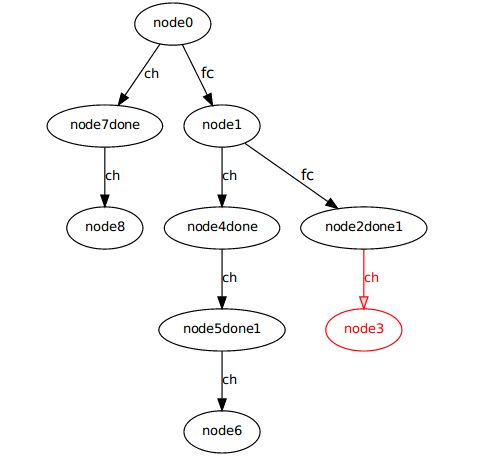
\includegraphics[scale=0.3]{p1.png}
  \begin{itemize}
  \item for every function containing begin (see handle* functions in code) 
  \item create a syncGraph with nodes defined by
  \item use of sync vars, begin fun, if else, loop etc.
  
  \end{itemize}
\end{frame}

\begin{frame}[plain]
  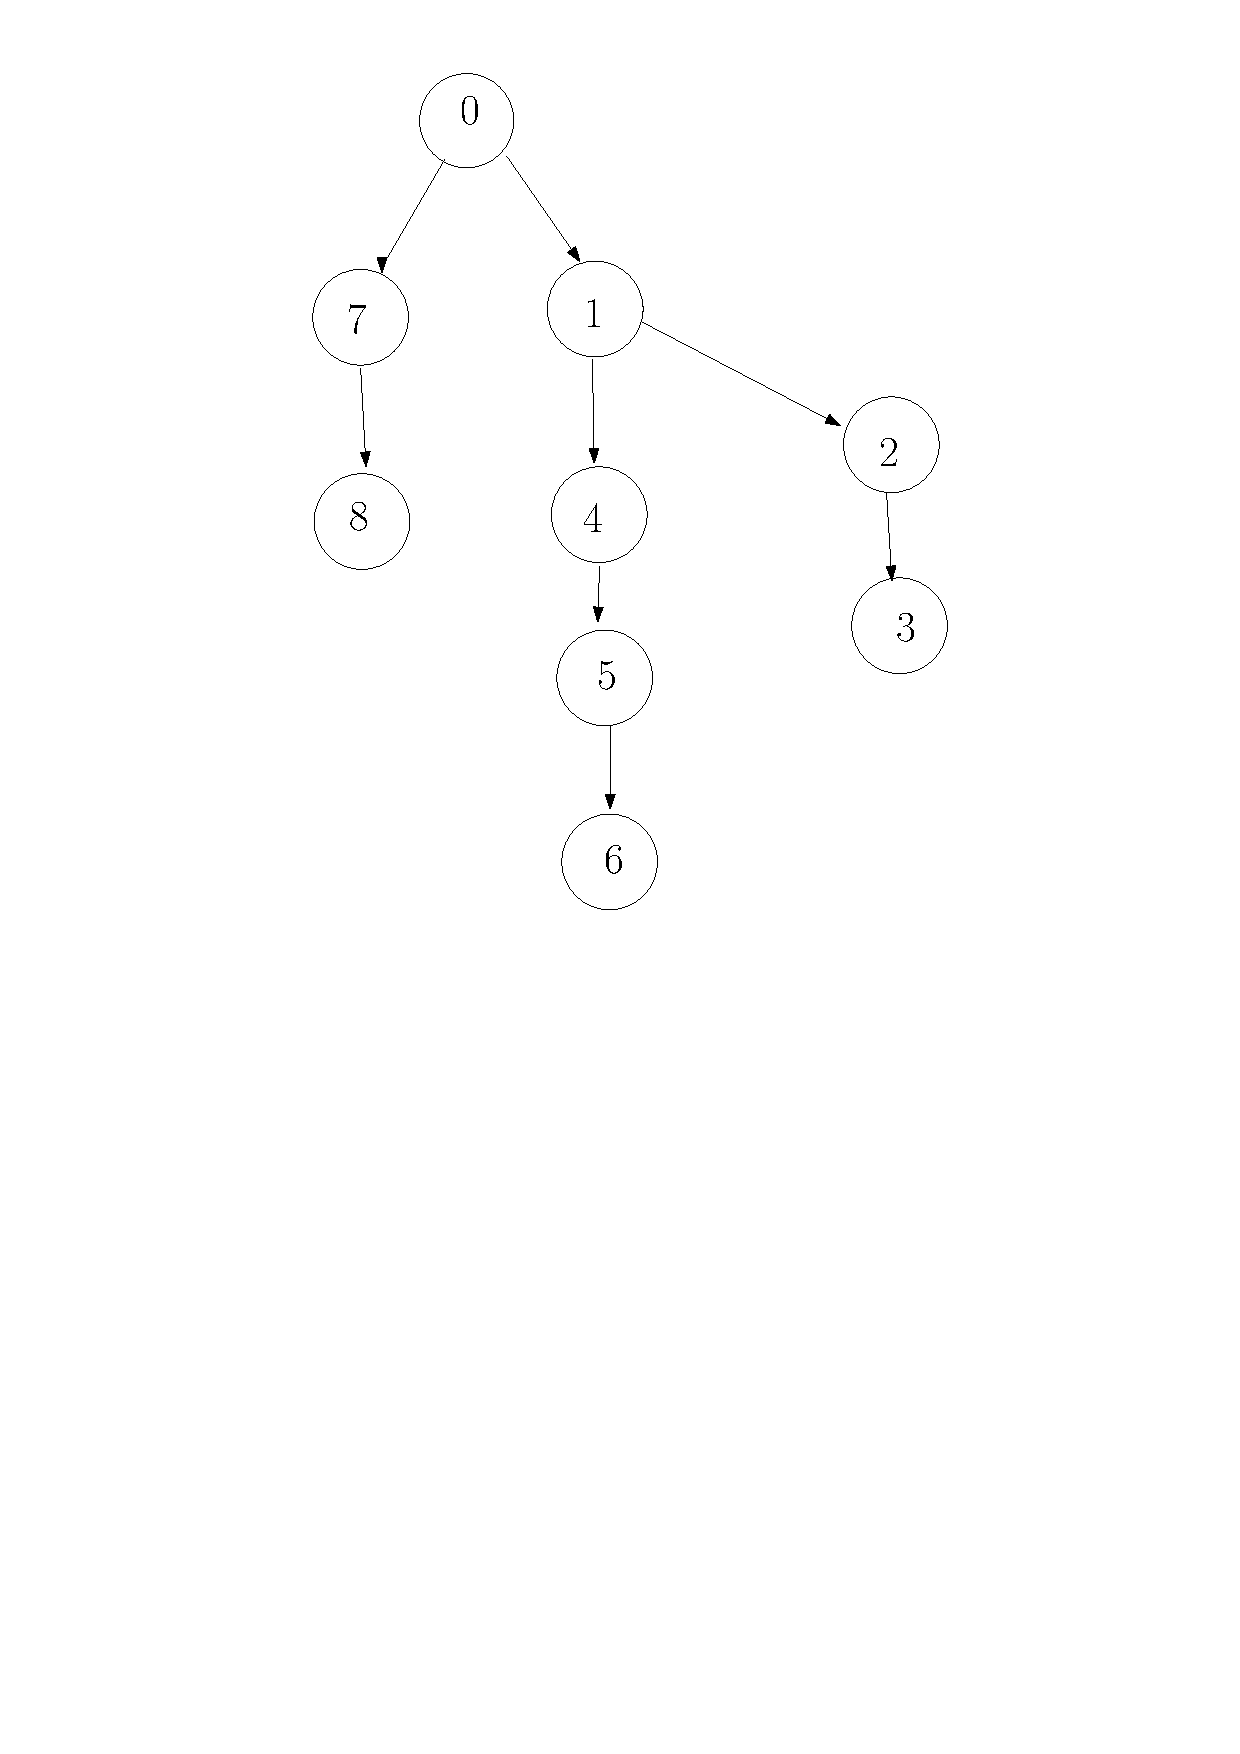
\includegraphics[scale=0.3]{start1.pdf}
  \begin{itemize}
  \item For each node save the use of external variables (UseInfo ). Here Node 1 \& 2
    uses external variable info.
  \end{itemize}
\end{frame}

\begin{frame}[plain]
  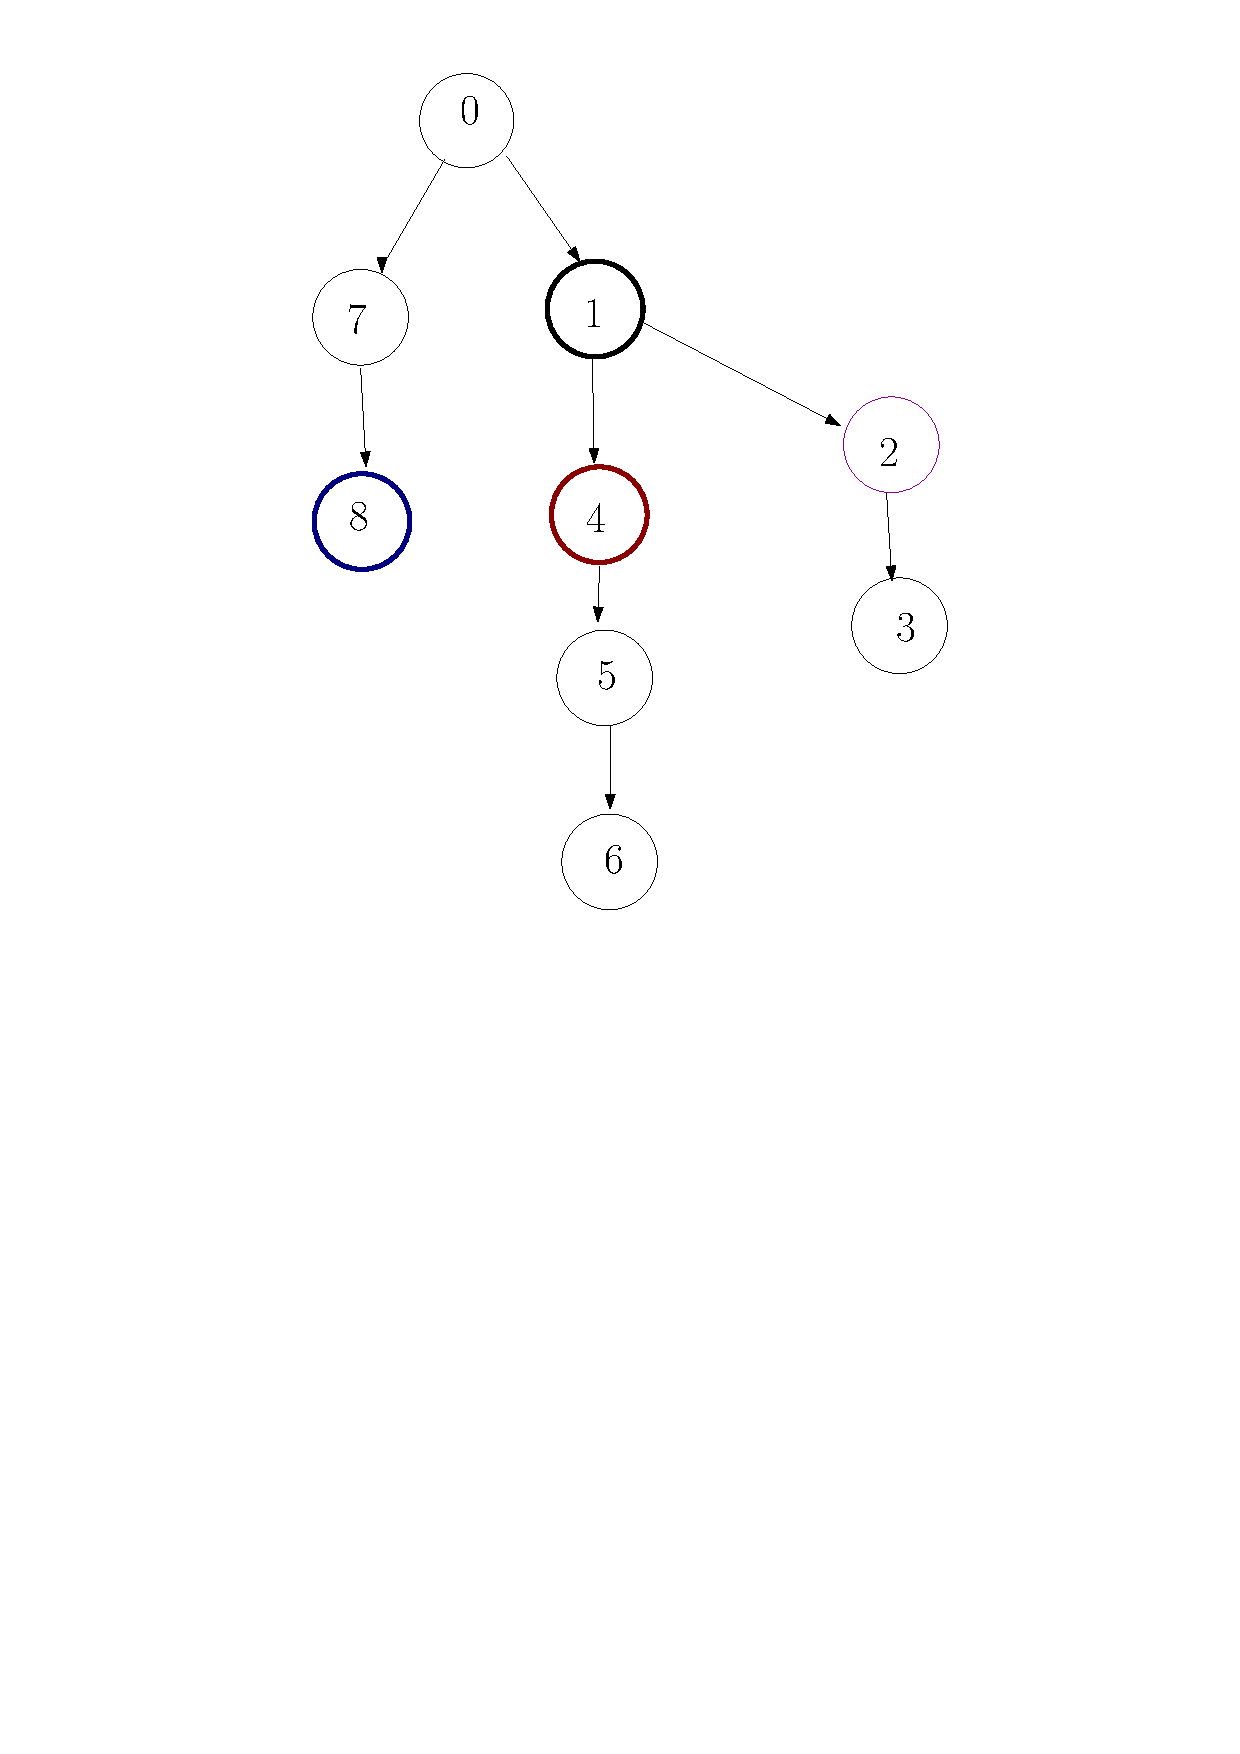
\includegraphics[scale=0.3]{start2.pdf}
  \begin{itemize}
  \item For each use save the next Dominated (should reach there through all paths)
    sync node in same Function and Last Sync Node
    in the Function of definition.(see setNextSyncNode, setLastSyncNode)
  \item For Node 1 it is Node 4 and Node 7 respectively.
  \end{itemize}
\end{frame}

\begin{frame}[plain]
  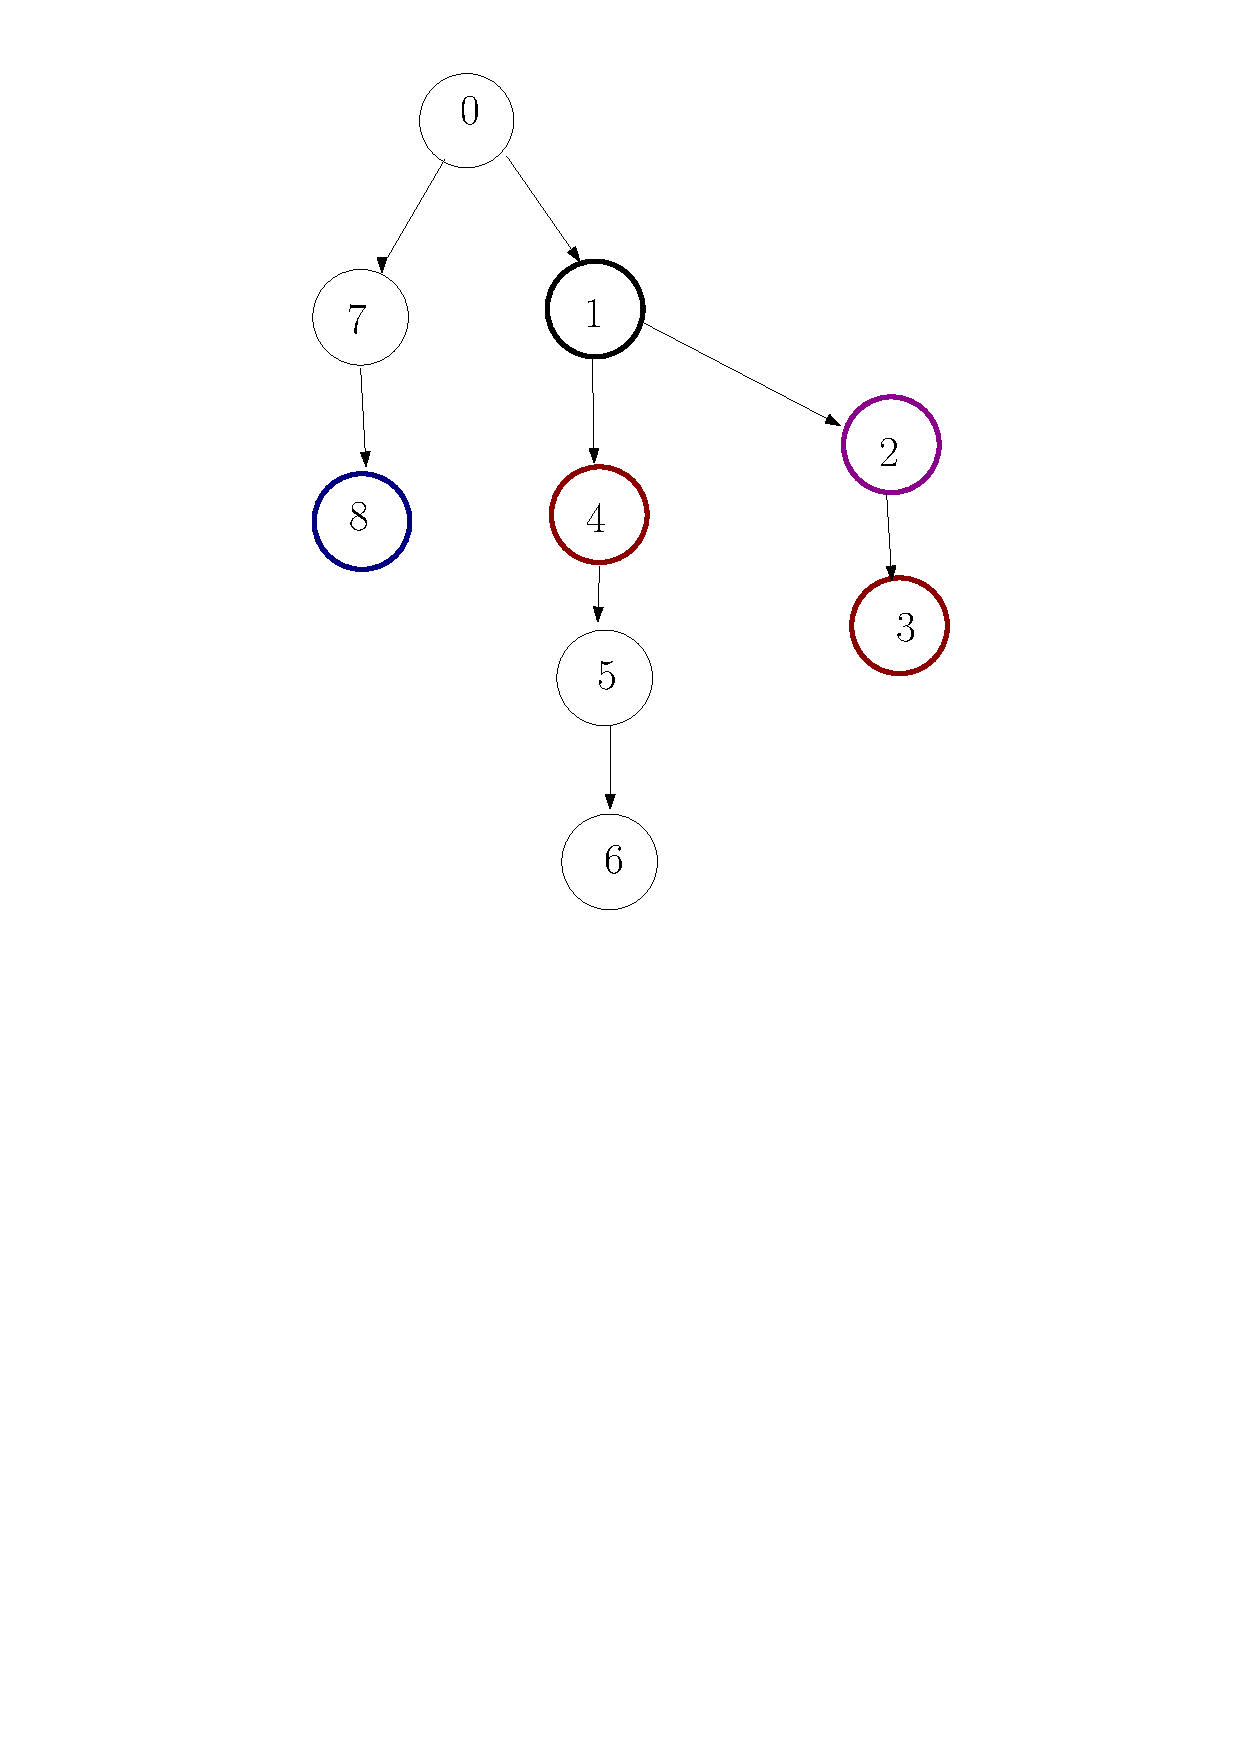
\includegraphics[scale=0.3]{start3.pdf}
  \begin{itemize}
  \item For Node 2 it is Node 2 and 7 respectively
  \item Our aim is to check if Node 7 can be passed before Node 2/ Node 4 is passed.
  \end{itemize}
\end{frame}

\begin{frame}[plain]
  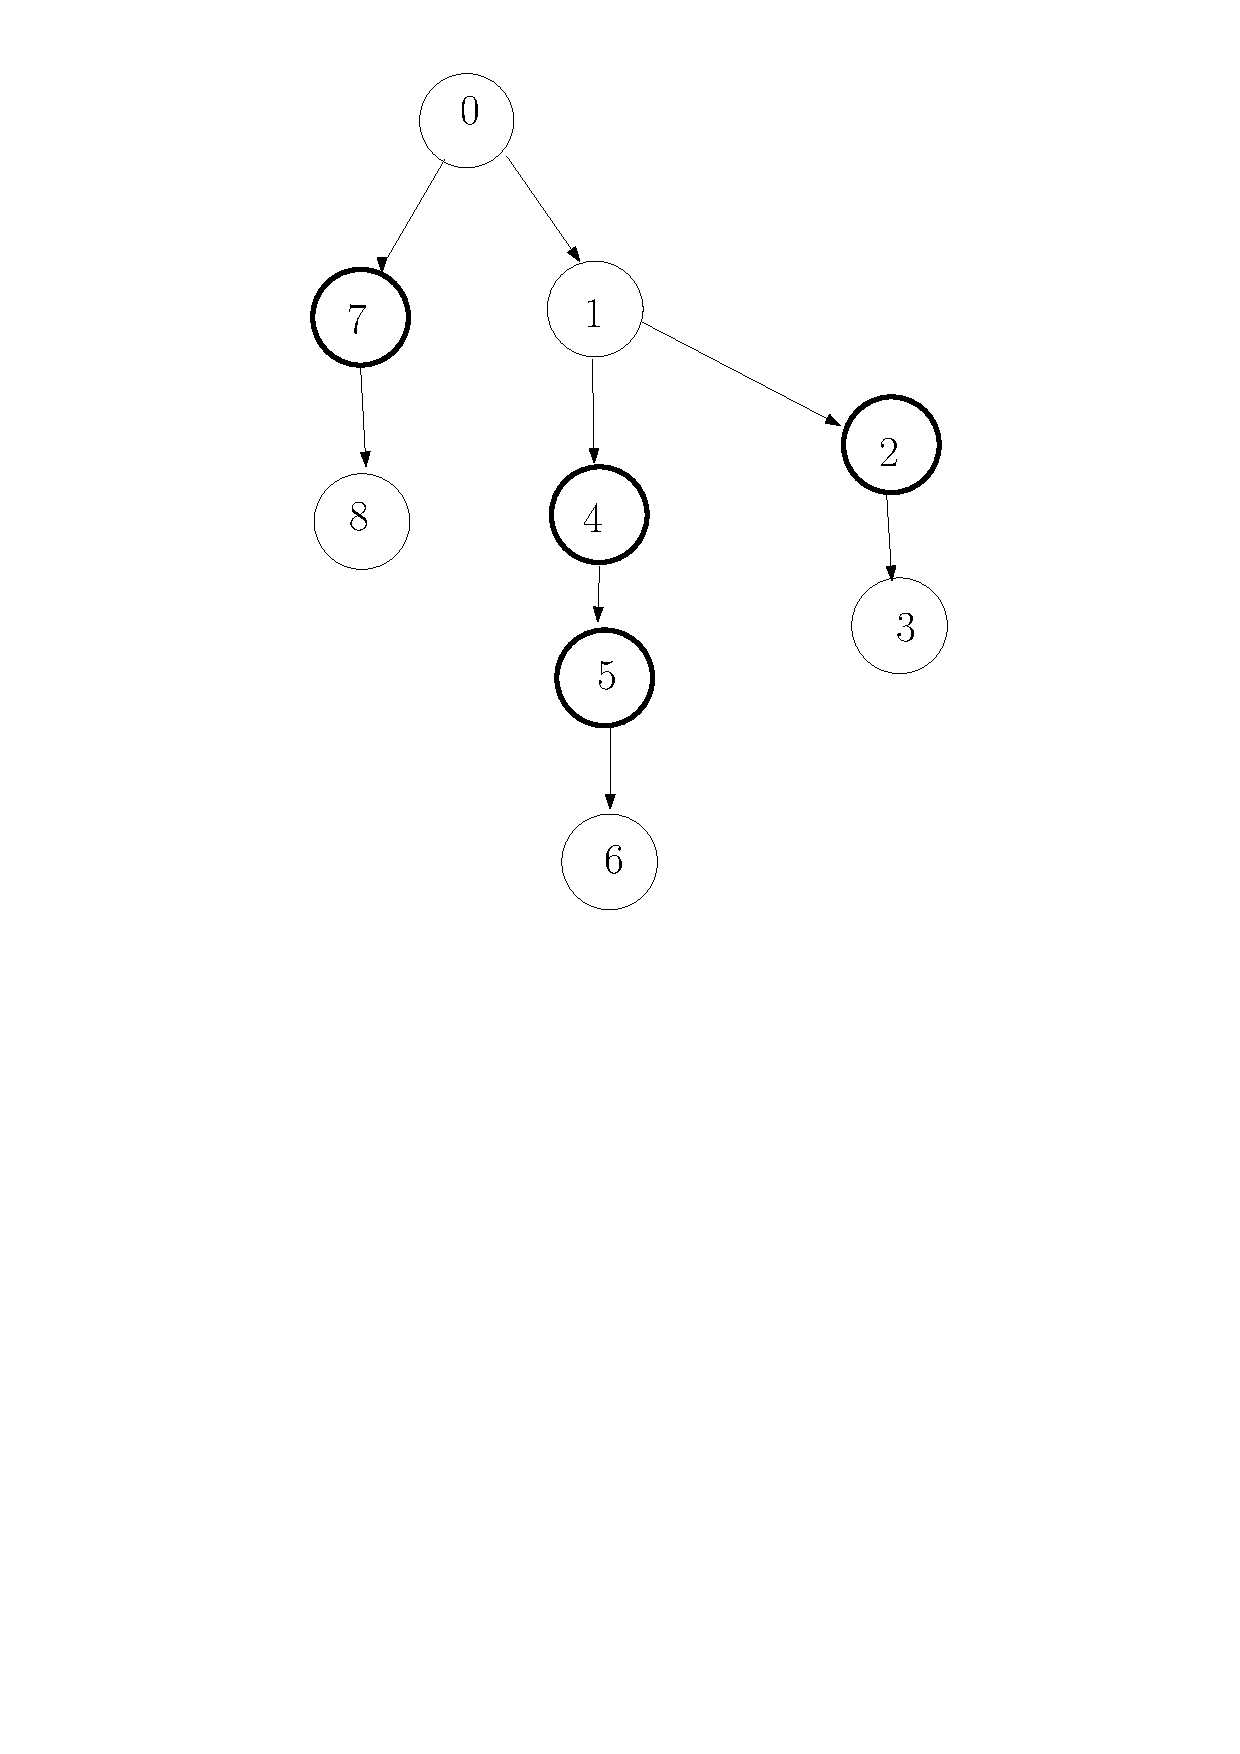
\includegraphics[scale=0.3]{syncpoints.pdf}
  \begin{itemize}
  \item The Graph has 4 sync points Nodes 2,4,5 7.
  \item Next id to find all possible set of Sync points that can be live at a given time.
    see(collectAllAvailableSyncPoints)
  \end{itemize}
\end{frame}


\begin{frame}[plain]
  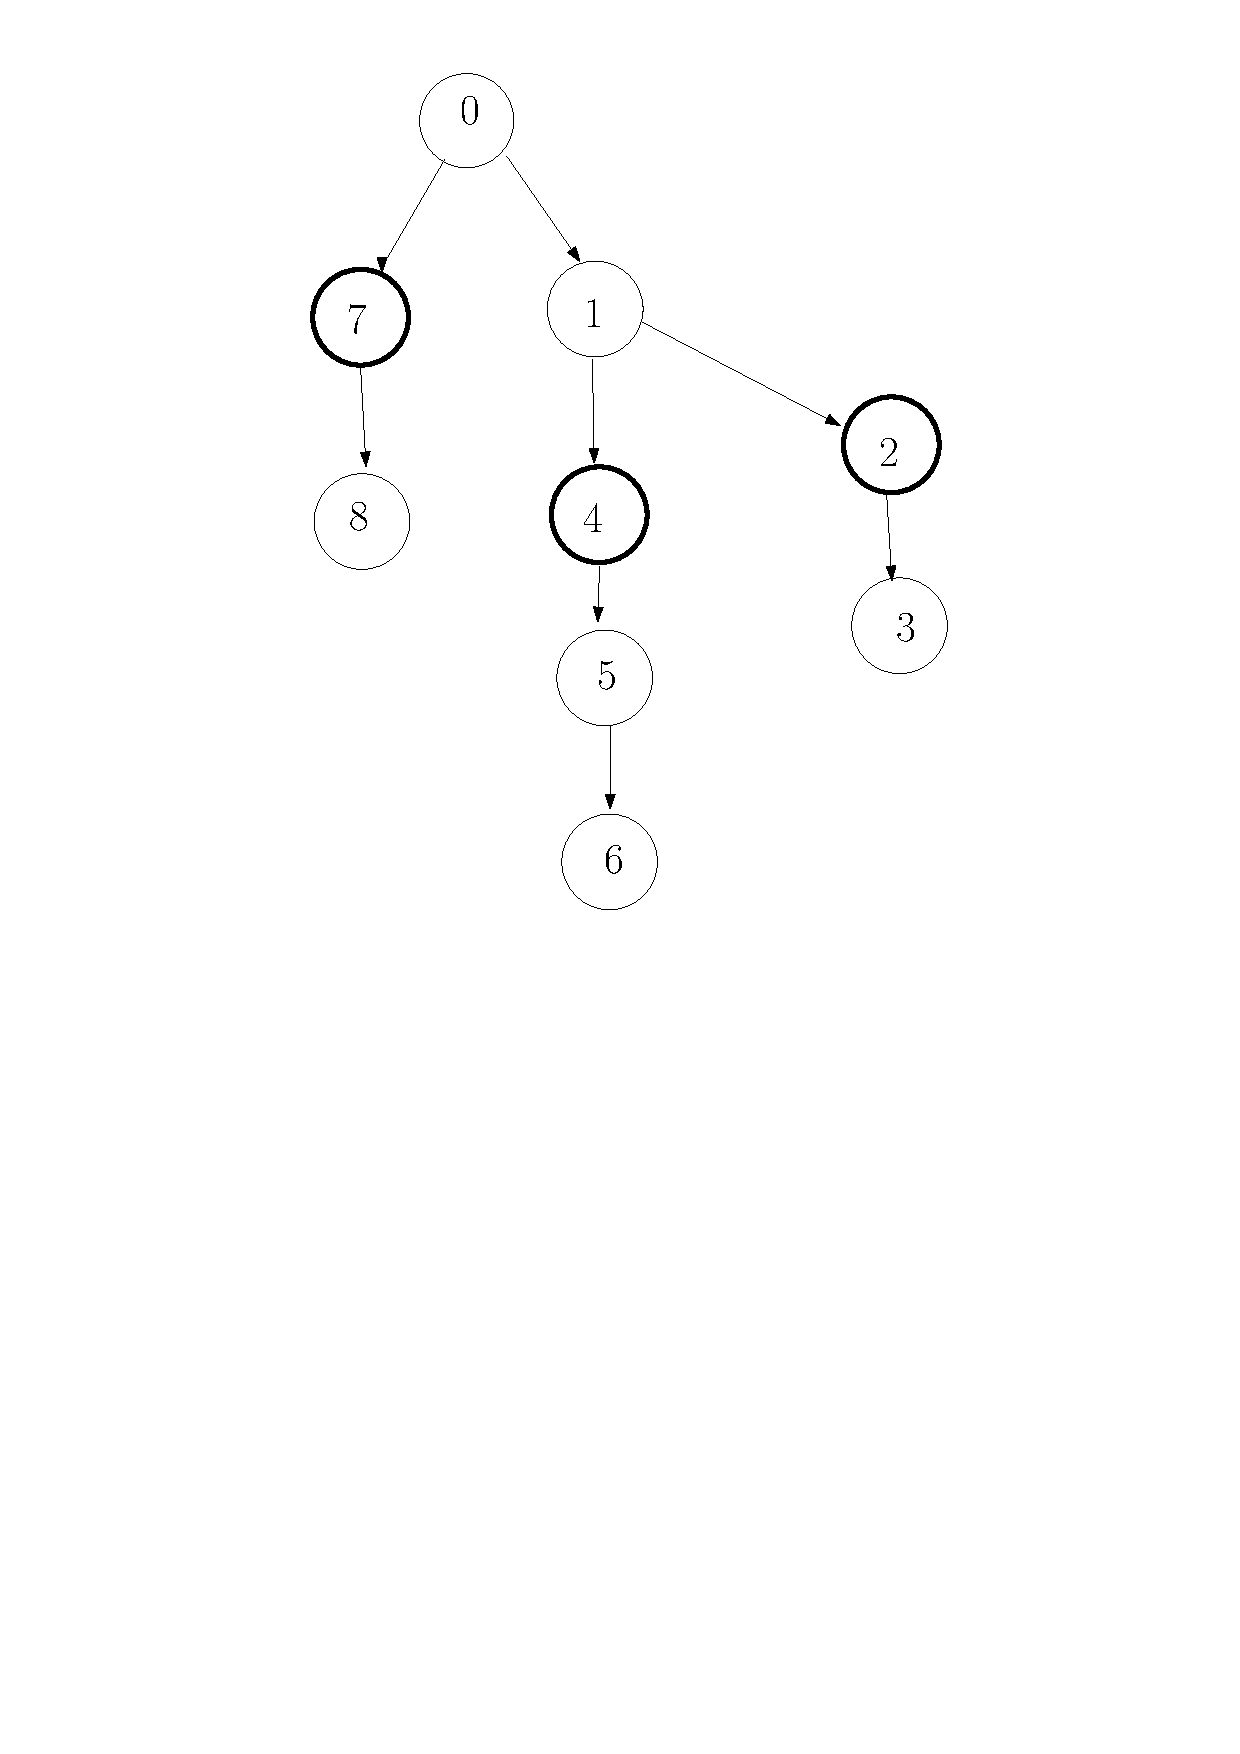
\includegraphics[scale=0.3]{VisitMap.pdf}
  \begin{itemize}
  \item Going through all paths we see 7,4,2 are the first set of sync points which are live.
  \item We add it to the list of possible sync points to set (see:VisitedMap).
  \item Now we try to see if there are sync Nodes that can be synchronized with each other.
    (see:threadedMahjong)
  \end{itemize}
\end{frame}


\begin{frame}[plain]
  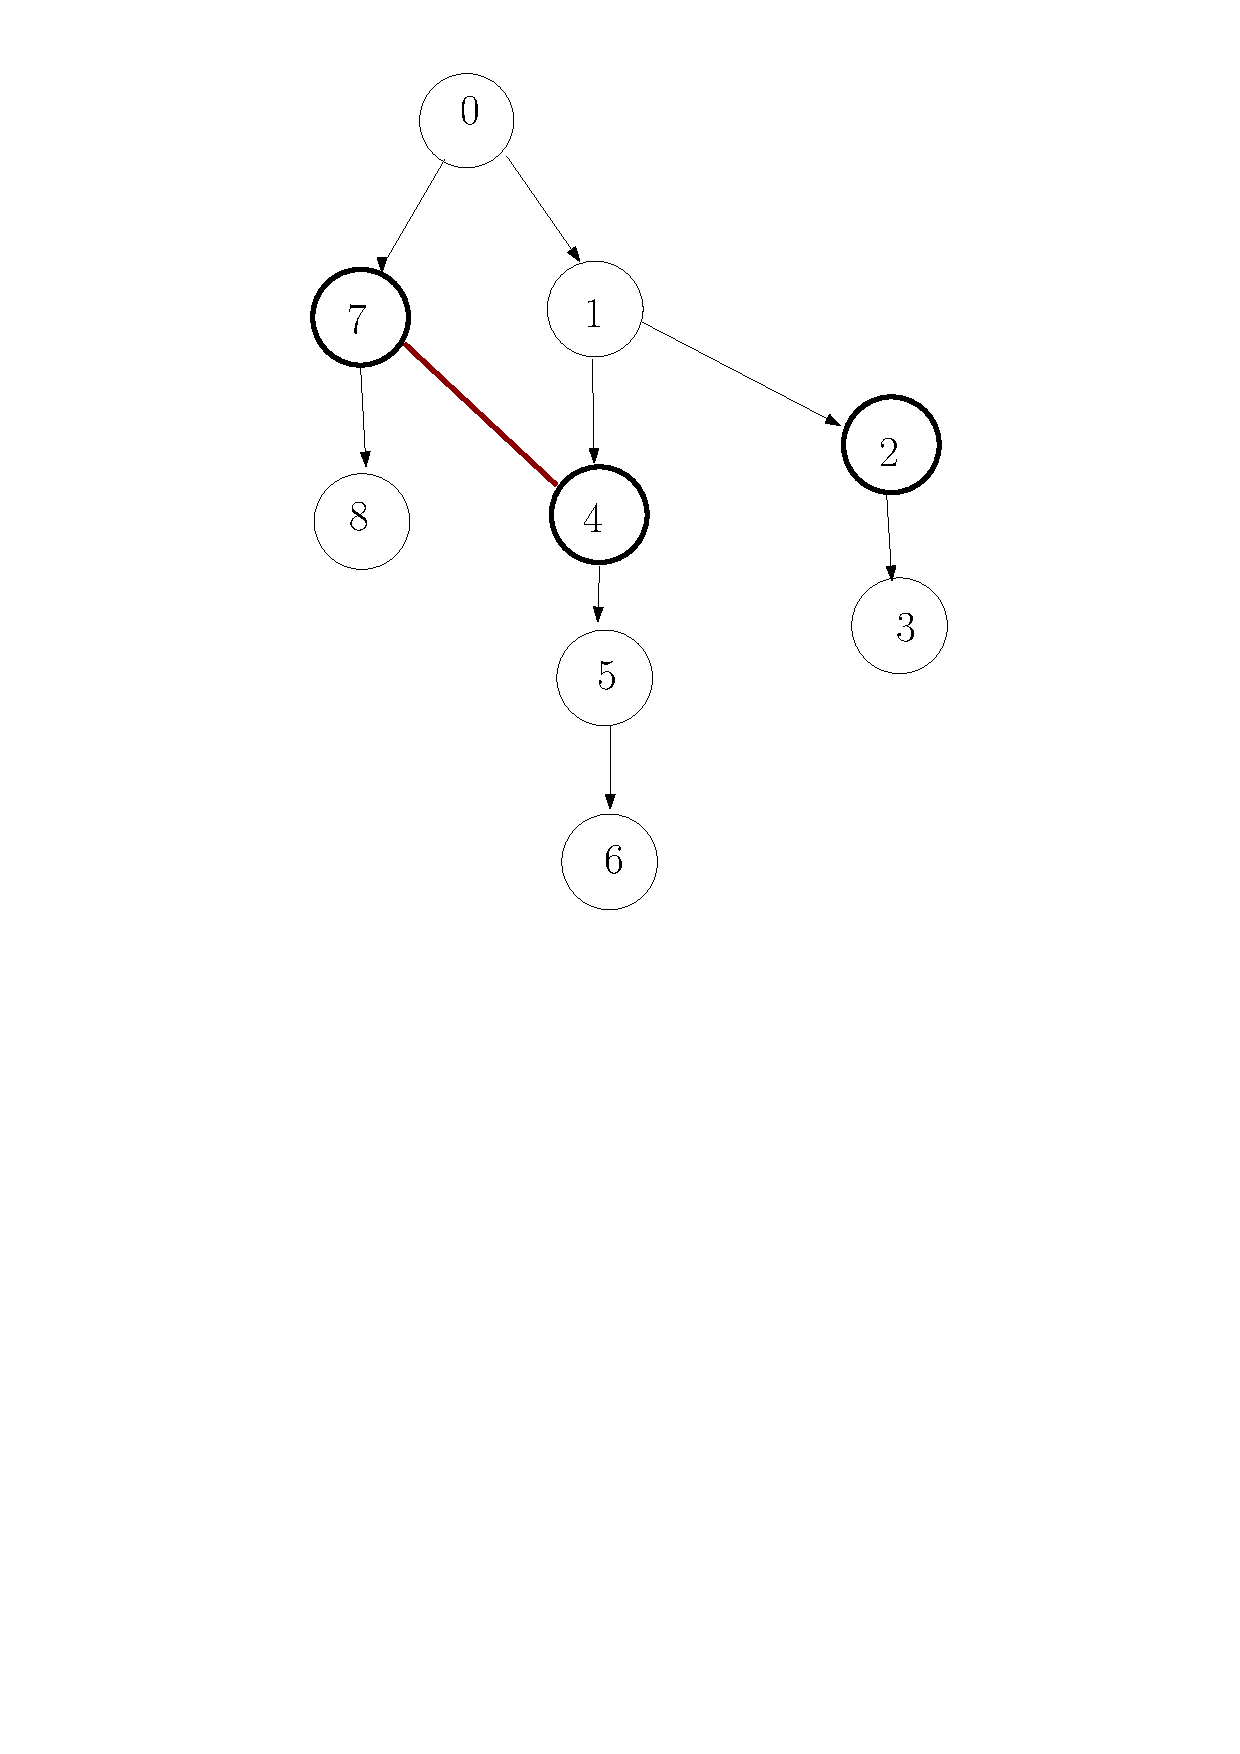
\includegraphics[scale=0.3]{firstMatch.pdf}
  \begin{itemize}
  \item Nodes 7 and 4 are matched.
  \end{itemize}
\end{frame}

\begin{frame}[plain]
  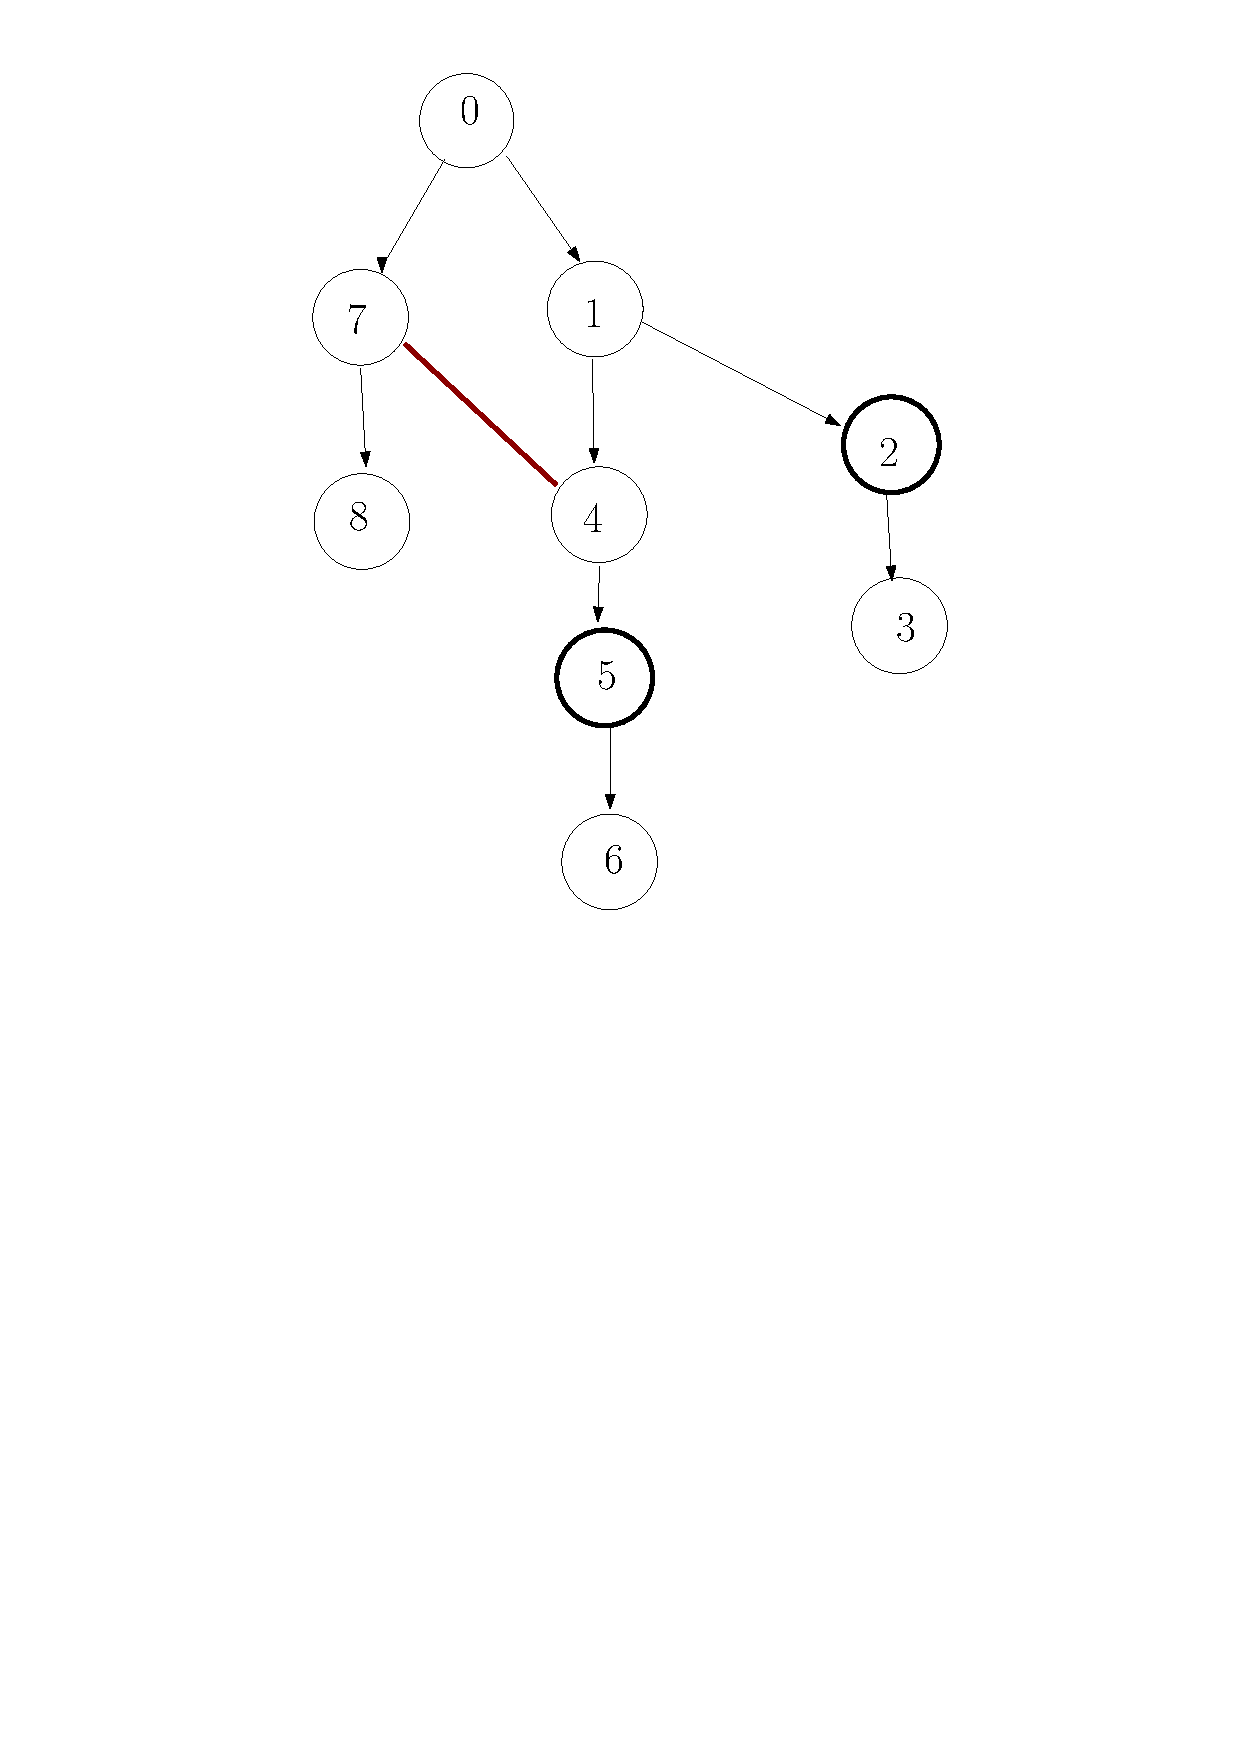
\includegraphics[scale=0.3]{VisitMap2.pdf}
  \begin{itemize}
  \item Now Node 5 becomes available. 
  \end{itemize}
\end{frame}


\begin{frame}[plain]
  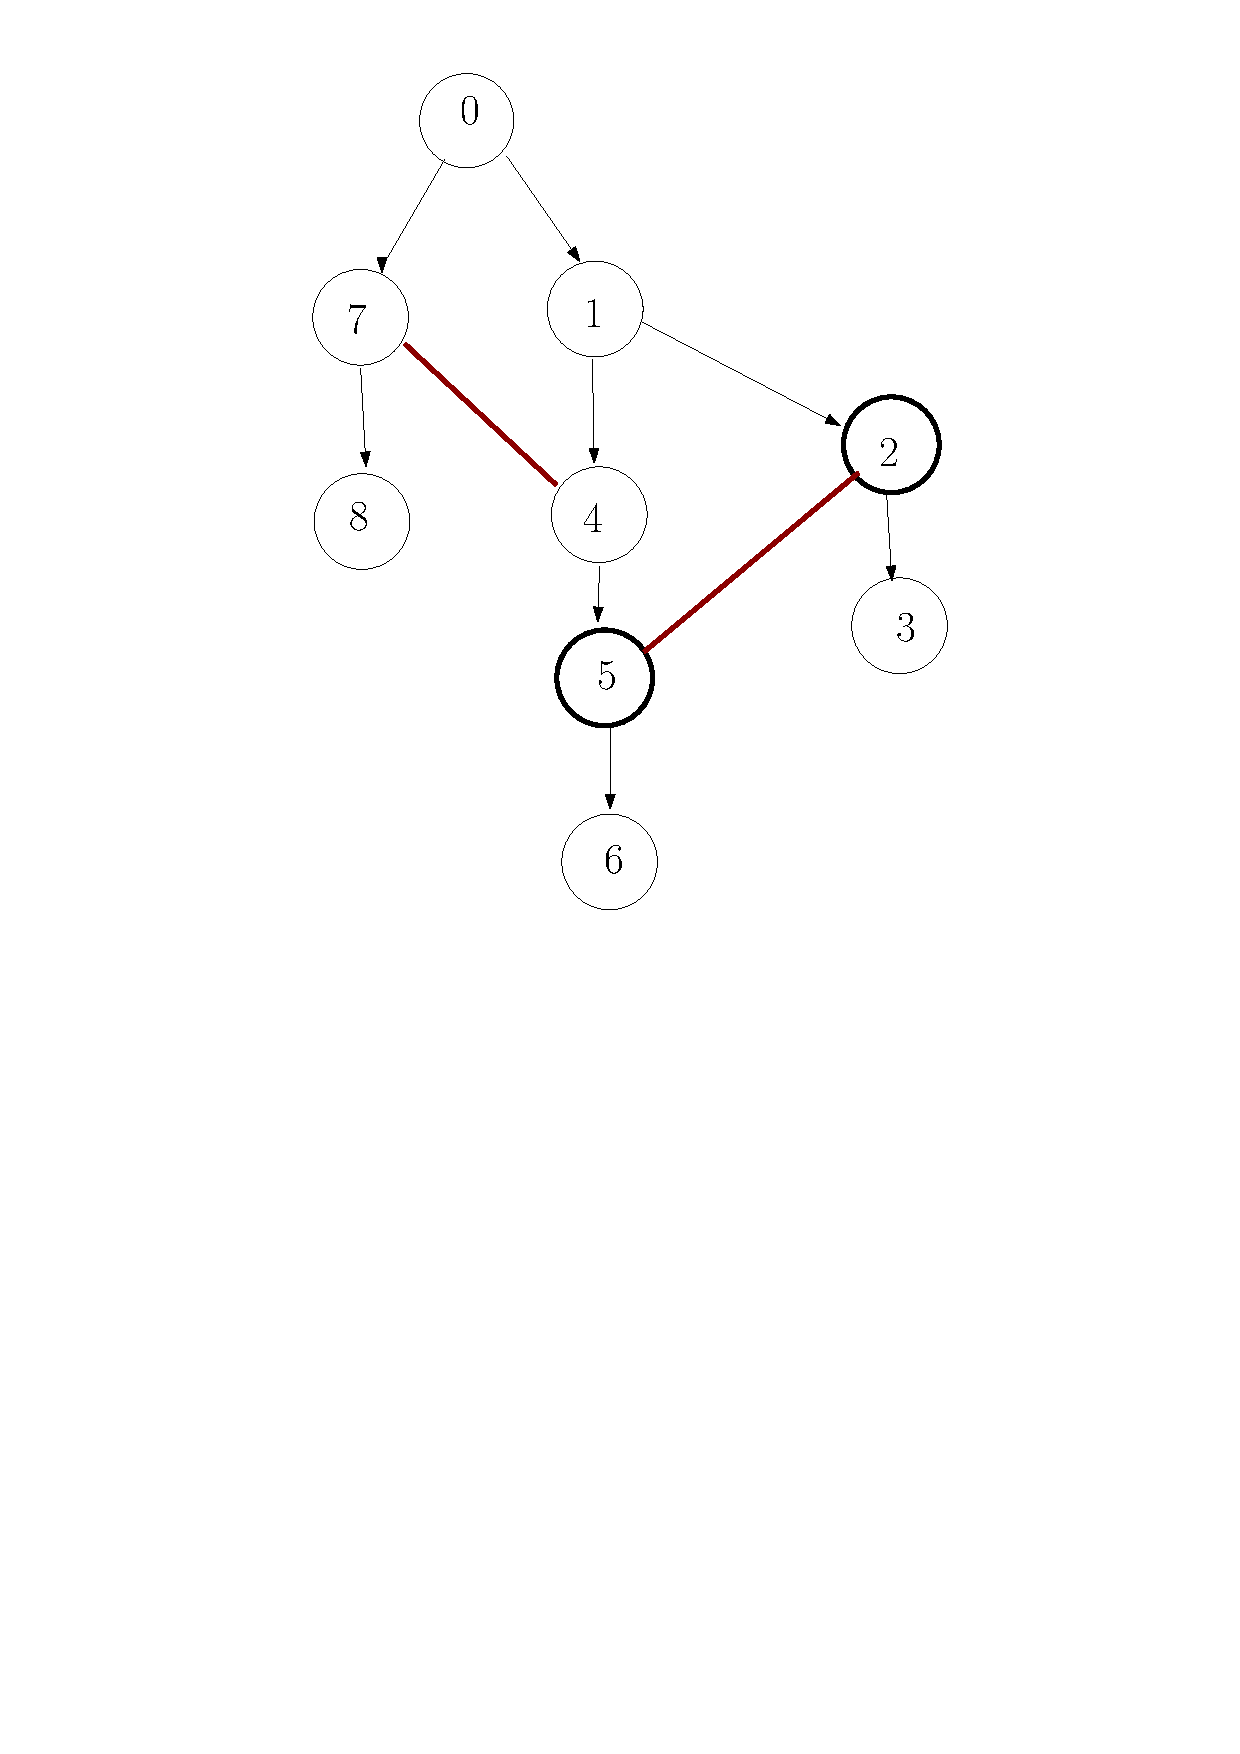
\includegraphics[scale=0.3]{syncPoints2.pdf}
  \begin{itemize}
  \item Nodes 2 and 5 are Matched.
  \end{itemize}
\end{frame}


\begin{frame}[plain]
  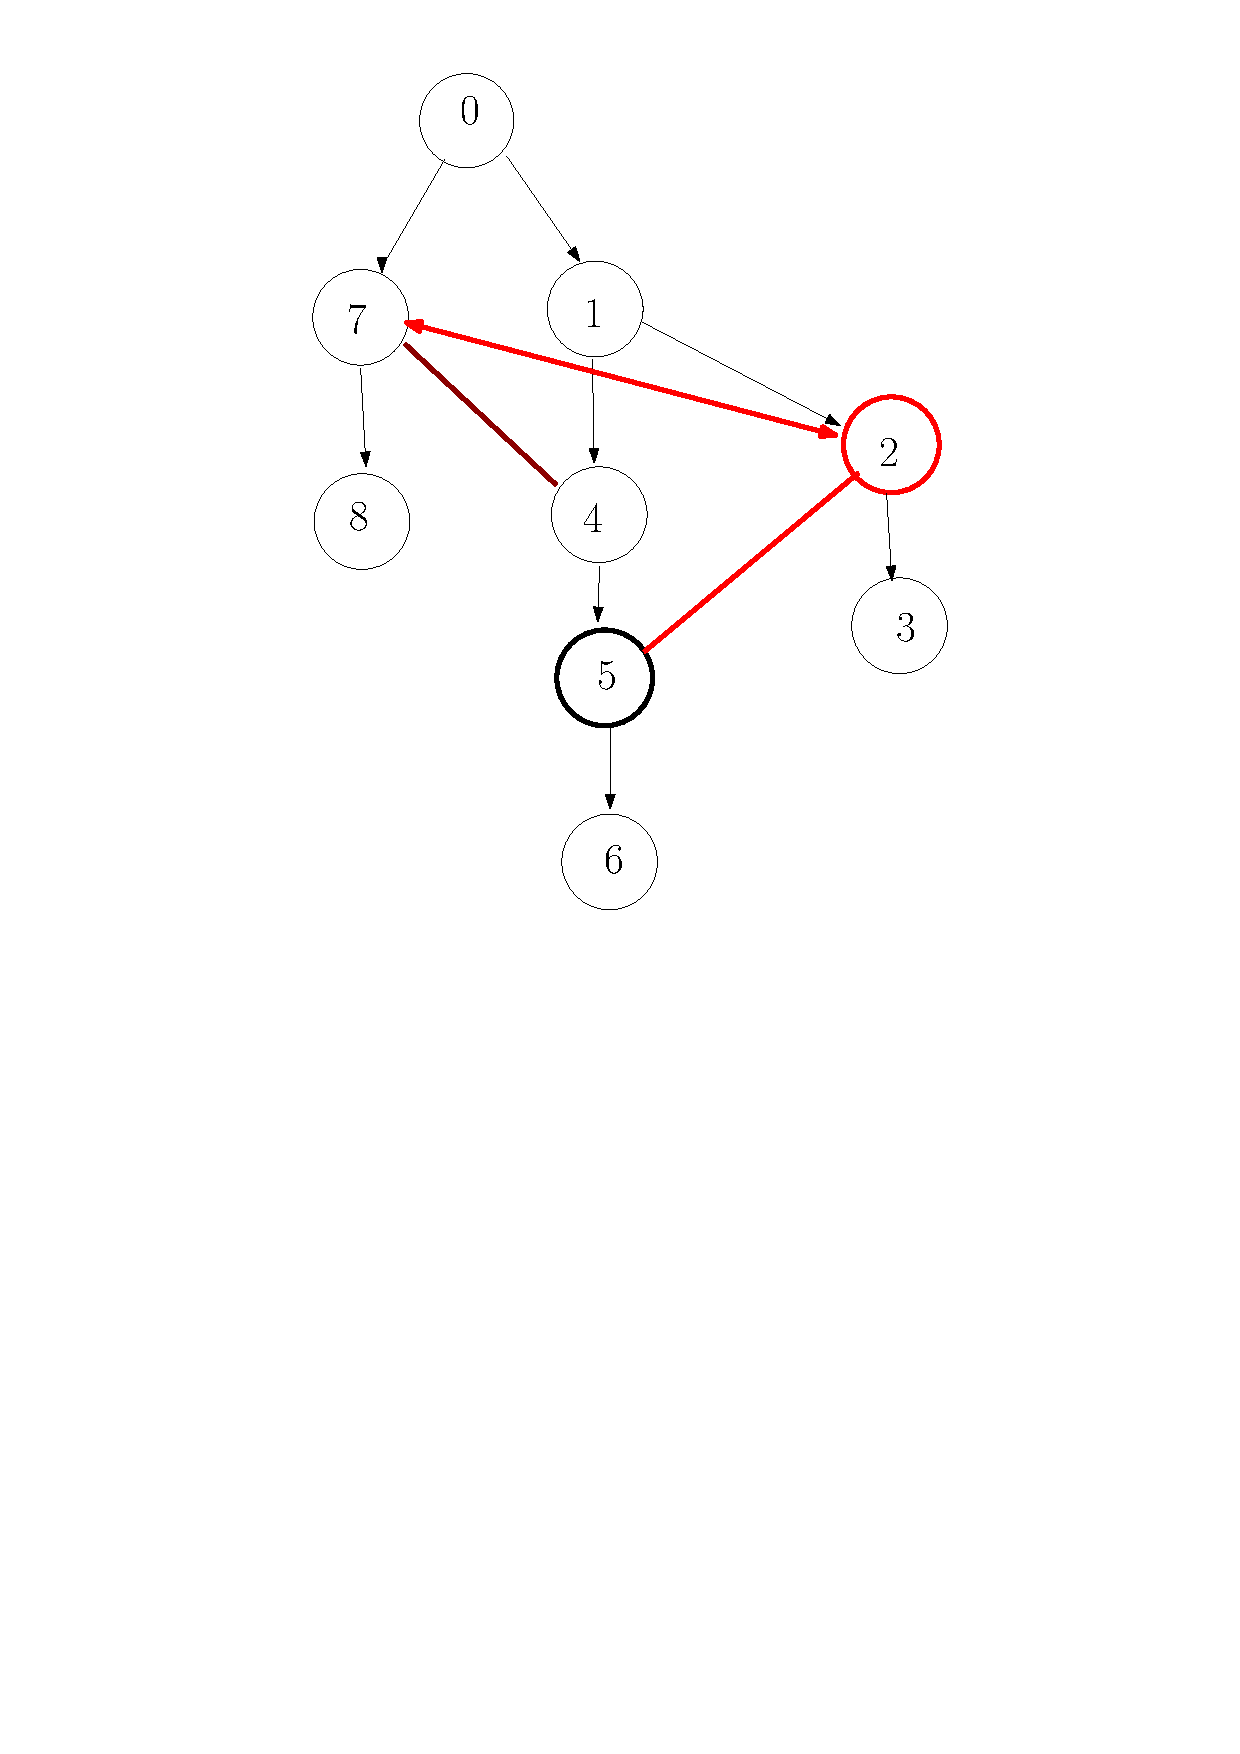
\includegraphics[scale=0.3]{checksyncPoints2.pdf}
  \begin{itemize}
  \item if a newly matched set contains a node which is set as nextSyncPoint.
    we check if lastSyncPoint is already visited. If yes Throw error.
   Since node 7 is already visited we throw error at use of variable at node 2. 
  \end{itemize}
\end{frame}



\begin{frame}[plain]
  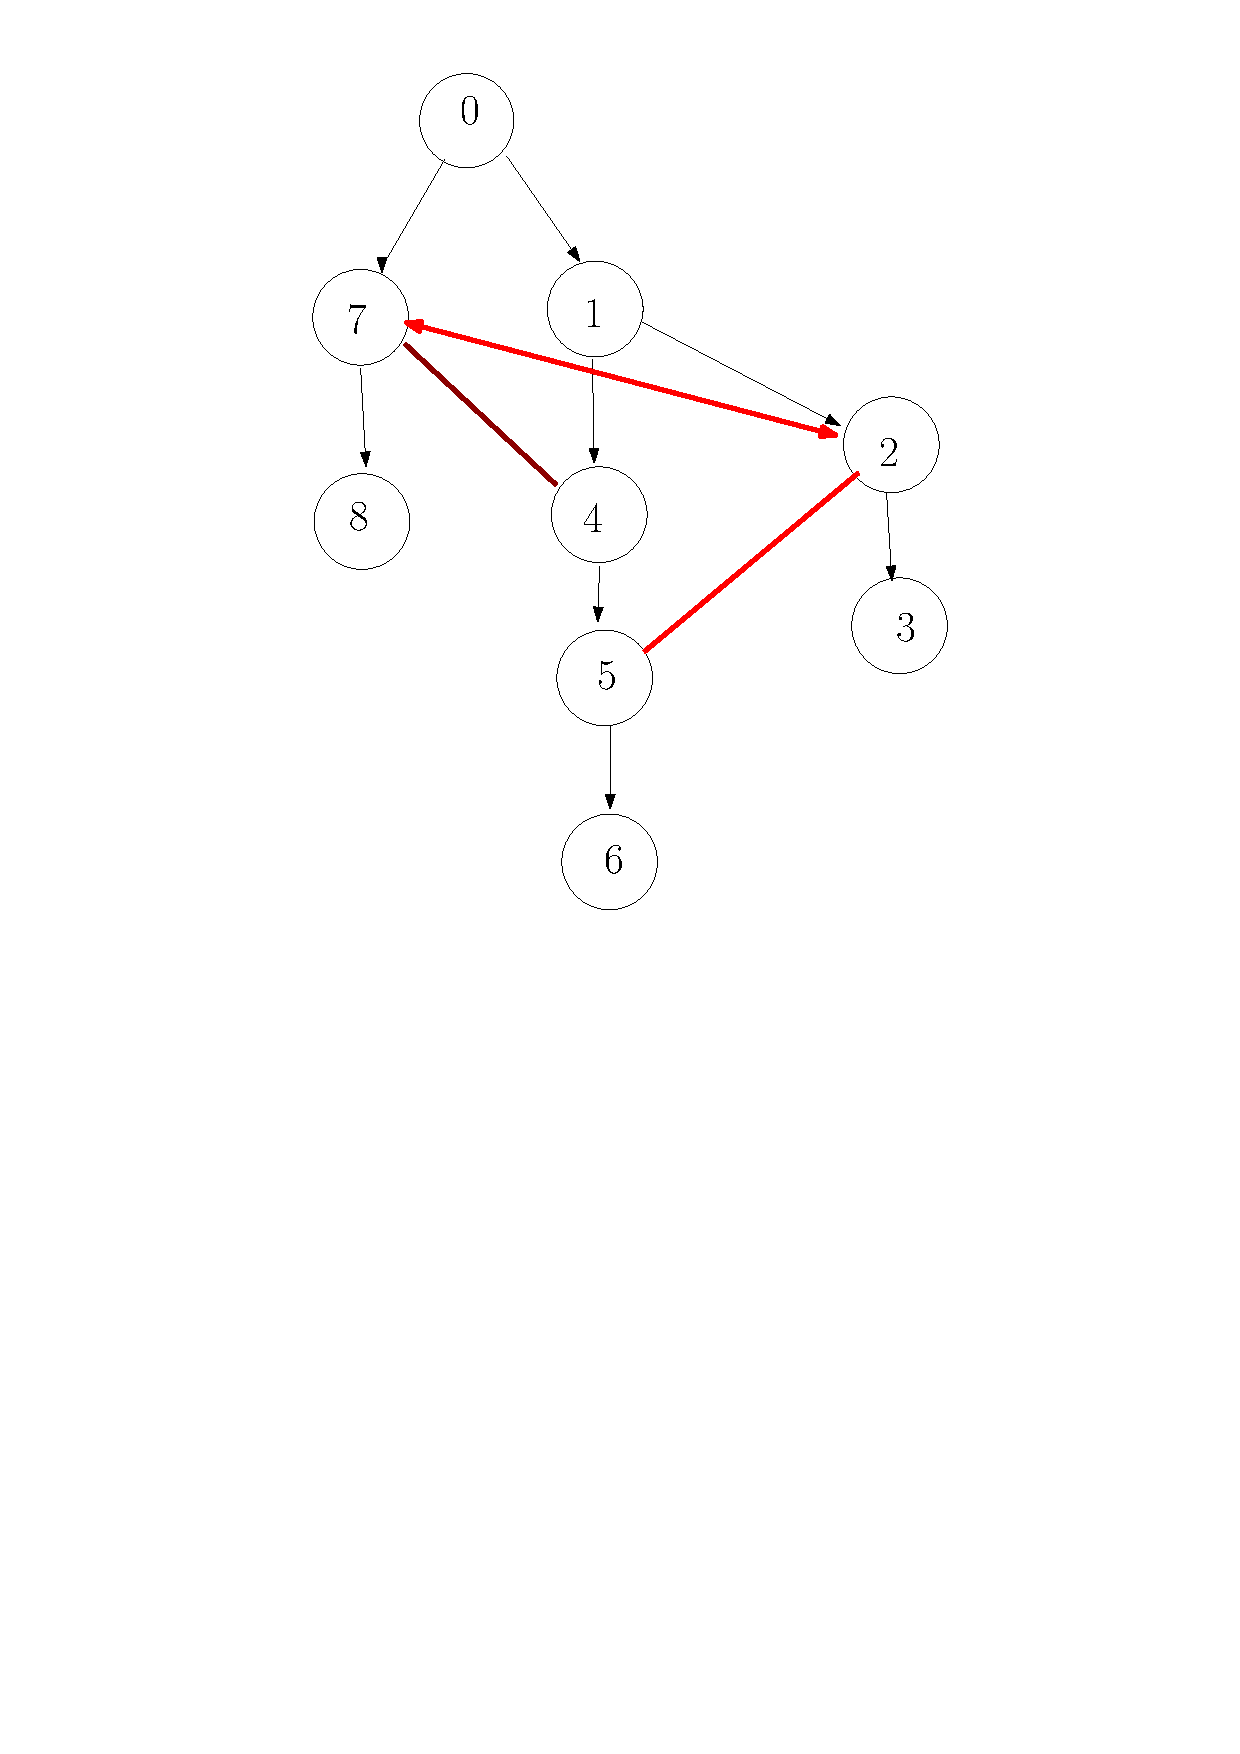
\includegraphics[scale=0.3]{end.pdf}
  \begin{itemize}
  \item No more sync point sets.
  \item delete and clean up. 
  \end{itemize}
\end{frame}



\begin{frame}[plain]
  \begin{itemize}
  \item for If-else : both paths are taken each given a different VisitMap config. If
    any one of them leads to error. we show the warning.
  \item for Internal Functions: inline the nodes of internal functions. Break as soon as we see
    recursion.
  \end{itemize}
\end{frame}


\end{document}
